\documentclass[twocolumn,10pt,a4paper]{article}
\usepackage[a4paper, top=1.8cm, bottom=1.8cm, left=1.5cm, right=1.5cm, columnsep=0.6cm]{geometry}
\usepackage{amsmath, amssymb, amsfonts}
\usepackage{graphicx}
\usepackage{booktabs}
\usepackage{microtype}
\usepackage{tikz}
\usetikzlibrary{arrows.meta, positioning, shapes, decorations.pathmorphing, calc}
\usepackage{caption}
\usepackage{subcaption}
\usepackage{titlesec}
\usepackage{enumitem}
\usepackage{cite}
\usepackage{flushend}
\usepackage[colorlinks=true, linkcolor=blue, citecolor=blue, urlcolor=blue]{hyperref}

% Global List Formatting
\setlist{topsep=2pt, itemsep=1.5pt, parsep=0pt, partopsep=0pt}

% Typography & Section Formatting
\titleformat{\section}{\large\bfseries}{\thesection.}{0.5em}{}
\titleformat{\subsection}{\normalsize\bfseries}{\thesubsection.}{0.5em}{}
\titleformat{\subsubsection}{\small\bfseries}{\thesubsubsection.}{0.5em}{}
\titlespacing*{\section}{0pt}{1.0ex plus 0.3ex minus 0.2ex}{0.4ex}
\titlespacing*{\subsection}{0pt}{0.8ex plus 0.2ex minus 0.2ex}{0.3ex}
\titlespacing*{\subsubsection}{0pt}{0.6ex plus 0.2ex minus 0.1ex}{0.2ex}

\captionsetup{font=small, labelfont=bf, skip=4pt}

\title{\LARGE\textbf{Experimental and Computational Investigation of Optical Rotatory Dispersion and the Barber Pole Effect in Chiral Media}}

\author{
  \textbf{Kartik Khare}\quad \textbf{Aneesh Bhate}\quad \textbf{Dhairya Nisar}\quad \textbf{Gouri Mittal}\\[0.3em]
  \textit{Department of Physics, Indian Institute of Technology}\\
  \textit{PH3050: Engineering Optics}
}
\date{\today}

\begin{document}

\twocolumn[
  \begin{@twocolumnfalse}
    \maketitle
    \begin{abstract}
      When linearly polarized polychromatic light propagates axially through a chiral, optically active fluid contained within a transparent cylinder, a striking visual phenomenon emerges: vivid, rainbow-colored helical stripes wind around the tube wall when viewed transversely. This manifestation, commonly termed the \textit{Barber Pole Effect}, arises from the physical interplay between circular birefringence, wavelength-dependent optical activity (Optical Rotatory Dispersion, ORD), and transverse Rayleigh dipole scattering. In this work, we present a rigorous theoretical framework, a detailed experimental apparatus design, and high-fidelity volumetric computational simulations of the effect using concentrated aqueous D-glucose solutions. We demonstrate analytically and numerically that the spatial helical pitch scales quadratically with wavelength ($P(\lambda) \propto \lambda^2$) as a consequence of Cauchy's rotatory dispersion law ($\theta \propto 1/\lambda^2$), and we experimentally formulate the conditions under which rotating the entrance polarizer induces a continuous apparent axial translation of the stripes (\textit{walking stripes}). Furthermore, we validate Biot's law through linear inverse-square regressions, examine the Malus analyzer transmission spectra, and elucidate the perceptual color de-saturation governing continuous broadband illumination.
      \vspace{0.8em}
    \end{abstract}
  \end{@twocolumnfalse}
]

\section{Introduction \& Theoretical Background}

Optical activity—the spontaneous rotation of the plane of linear polarization as electromagnetic waves traverse chiral matter—was first documented by Jean-Baptiste Biot in 1815 and theoretically explained by Augustin-Jean Fresnel in 1822 \cite{biot1815, fresnel1822}. Beyond standard polarimetric concentration assays, optical activity exhibits rich spatial and chromatic behavior when coupled with transverse light scattering in macroscopic fluid volumes.

\subsection{Circular Birefringence \& Polarimetric Rotation}
Chiral molecules, such as D-glucose (dextrose), lack improper rotation axes ($S_n$), resulting in non-centrosymmetric helical molecular charge distributions. When an electromagnetic plane wave interacts with such stereocenters, the medium responds differently to right-circularly polarized (RCP, $\hat{e}_+$) and left-circularly polarized (LCP, $\hat{e}_-$) fields, exhibiting \textit{circular birefringence}:
\begin{equation}
  \Delta n(\lambda) = n_L(\lambda) - n_R(\lambda) \neq 0
  \label{eq:circ_birefringence}
\end{equation}
Any linearly polarized plane wave propagating along the $z$-axis with initial polarization orientation $\theta_0$ can be expressed as a coherent superposition of circular eigenmodes:
\begin{equation}
  \vec{E}(0, t) = \frac{E_0}{\sqrt{2}} \left( \hat{e}_+ e^{i\theta_0} + \hat{e}_- e^{-i\theta_0} \right) e^{-i\omega t}
  \label{eq:e_field_decomposition}
\end{equation}
where $\hat{e}_\pm = (\hat{x} \pm i\hat{y})/\sqrt{2}$. Upon propagating through an optical path length $z$, the two eigenmodes accumulate differing wavevectors $k_R = 2\pi n_R / \lambda_0$ and $k_L = 2\pi n_L / \lambda_0$. Recombining the propagated modes yields:
\begin{align}
  \vec{E}(z, t) &= E_0 e^{i(\bar{k}z - \omega t)} \left[ \hat{x} \cos\theta(z) + \hat{y} \sin\theta(z) \right] \label{eq:rotated_e_field} \\
  \theta(z) &= \theta_0 + \rho \cdot z = \theta_0 + \frac{\pi}{\lambda_0}(n_L - n_R)z
  \label{eq:rot_angle}
\end{align}
where $\bar{k} = (k_R + k_L)/2$. The output remains strictly linearly polarized, but its polarization azimuth rotates steadily with path length $z$ at a rotatory rate $\rho = d\theta/dz$.

\subsection{Biot's Law \& Cauchy Rotatory Dispersion}
For a dilute or moderately concentrated solution of chiral solute in an optically inactive solvent, Biot's law dictates that the rotation angle $\theta$ is directly proportional to the solute mass concentration $c$ and propagation distance $z$ \cite{biot1815}:
\begin{equation}
  \theta(\lambda) = [\alpha]_\lambda^T \cdot c \cdot z
  \label{eq:biot_law}
\end{equation}
where $[\alpha]_\lambda^T$ is the specific rotation at temperature $T$ and wavelength $\lambda$. 

Away from electronic molecular resonance bands (the ultraviolet Cotton effect), the circular birefringence $\Delta n(\lambda)$ follows Augustin-Louis Cauchy's normal dispersion expansion \cite{cauchy1836, djerassi1960}:
\begin{equation}
  \rho(\lambda) = \frac{\theta}{c \cdot z} \approx \frac{A}{\lambda^2} + \frac{B}{\lambda^4} + \dots
  \label{eq:cauchy_dispersion}
\end{equation}
Retaining the leading-order term yields the fundamental governing equation of Optical Rotatory Dispersion (ORD) in our system:
\begin{equation}
  \theta(z, \lambda) = \theta_0 + \frac{A \cdot c \cdot z}{\lambda^2}
  \label{eq:cauchy_governing}
\end{equation}
where $A \approx 2.1 \times 10^6\,\text{nm}^2\cdot\text{rad}\cdot\text{cm}^{-1}\cdot(\text{g/cm}^3)^{-1}$ for concentrated aqueous D-glucose. Because $\theta \propto 1/\lambda^2$, violet light ($\lambda \approx 400\,\text{nm}$) rotates more than three times as rapidly as red light ($\lambda \approx 700\,\text{nm}$):
\begin{equation}
  \frac{\theta_{\text{violet}}(400\,\text{nm})}{\theta_{\text{red}}(700\,\text{nm})} = \left( \frac{700}{400} \right)^2 \approx 3.06
  \label{eq:dispersion_ratio}
\end{equation}

\subsection{Rayleigh Dipole Scattering Mechanism}
The visual manifestation of the barber pole pattern depends entirely on transverse observation. Suspended solute molecules or micro-particles within the liquid act as Rayleigh scatterers \cite{hecht2017}:
\begin{enumerate}[leftmargin=*]
  \item The incident local electric field $\vec{E}(z, \lambda)$ induces an oscillating dipole moment $\vec{p}(z, \lambda) = \alpha \vec{E}(z, \lambda)$ parallel to the electric field vector.
  \item Classical electrodynamics establishes that an oscillating dipole emits zero radiation along its dipole axis. The scattered radiant intensity $I$ along an arbitrary viewing unit vector $\hat{n}_{\text{view}}$ satisfies:
  \begin{equation}
    I \propto |\vec{p} \times \hat{n}_{\text{view}}|^2 = |\vec{p}|^2 \sin^2\psi
    \label{eq:dipole_pattern}
  \end{equation}
  where $\psi$ is the angle between the dipole orientation $\vec{p}$ and the observer's line of sight.
  \item When observing the tube horizontally in the transverse plane at viewing azimuth $\phi_{\text{view}}$, the observed intensity becomes:
  \begin{equation}
    I(z, \lambda) \propto \cos^2\left(\theta(z, \lambda) - \phi_{\text{view}}\right)
    \label{eq:transverse_intensity}
  \end{equation}
\end{enumerate}
Consequently, \textbf{extinction} ($I = 0$) occurs when the polarization vector points directly toward the observer ($\theta - \phi_{\text{view}} = \pm 90^\circ$), while \textbf{maximum emission} occurs when the polarization vector oscillates perpendicular to the line of sight ($\theta - \phi_{\text{view}} = 0^\circ, 180^\circ$). The fluid volume thus acts as a self-analyzing distributed polarimeter.

\subsection{Spatial Pitch \& The "Walking Stripes" Dynamics}
Because $\theta(z, \lambda)$ advances continuously along the cylinder, the maximum scattering locus forms a 3D helix. The axial distance for a complete $2\pi$ spatial turn defines the helical pitch $P(\lambda)$:
\begin{equation}
  P(\lambda) = \frac{2\pi \lambda^2}{A \cdot c}
  \label{eq:helical_pitch}
\end{equation}
Due to the $\cos^2$ intensity symmetry, the visible stripe repeats every half-pitch:
\begin{equation}
  P_{\text{stripe}}(\lambda) = \frac{\pi \lambda^2}{A \cdot c}
  \label{eq:stripe_pitch}
\end{equation}
Because $P(\lambda) \propto \lambda^2$, violet light establishes a tight, compressed spatial pitch ($P \approx 1.53\,\text{cm}$), whereas red light exhibits a stretched, elongated pitch ($P \approx 4.20\,\text{cm}$).

When the entrance linear polarizer is rotated at uniform angular frequency $\omega = d\theta_0 / dt$, the phase becomes time-dependent:
\begin{equation}
  \theta(z, \lambda, t) = \omega t + \frac{A \cdot c}{\lambda^2} z
  \label{eq:time_dep_phase}
\end{equation}
Imposing the constant phase condition ($d\theta = 0$) yields the apparent axial phase velocity of the stripes:
\begin{equation}
  v_{\text{phase}}(\lambda) = \frac{dz}{dt} = -\frac{\omega \lambda^2}{A \cdot c}
  \label{eq:phase_velocity}
\end{equation}
This confirms that rotating the entrance polarizer causes the helical stripes to glide continuously along the cylinder axis—the "walking stripes" illusion—without any physical fluid transport.

% Figure 1: Experimental Setup TikZ Diagram
\begin{figure}[t]
  \centering
  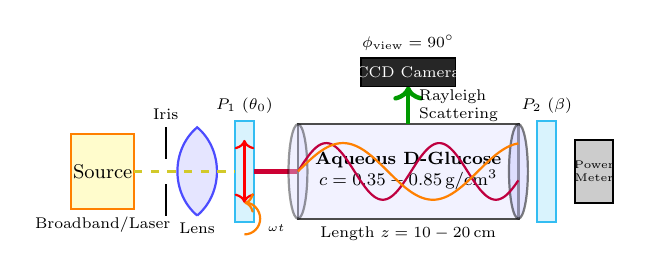
\begin{tikzpicture}[scale=0.80, every node/.style={transform shape}]
    % Light source
    \draw[fill=yellow!20, draw=orange, thick] (-0.8, -0.6) rectangle (0.2, 0.6);
    \node at (-0.3, 0) {\small Source};
    \node[below, font=\scriptsize] at (-0.3, -0.6) {Broadband/Laser};

    % Collimator / Iris
    \draw[fill=gray!30, thick] (0.7, 0.2) -- (0.7, 0.7);
    \draw[fill=gray!30, thick] (0.7, -0.2) -- (0.7, -0.7);
    \node[above, font=\scriptsize] at (0.7, 0.7) {Iris};

    % Collimating Lens
    \draw[fill=blue!10, draw=blue!70, thick] (1.2, -0.7) to[out=40, in=-40] (1.2, 0.7) to[out=220, in=140] (1.2, -0.7);
    \node[below, font=\scriptsize] at (1.2, -0.7) {Lens};

    % Polarizer P1
    \draw[fill=cyan!15, draw=cyan!80, thick] (1.8, -0.8) rectangle (2.1, 0.8);
    \draw[thick, <->, red] (1.95, -0.5) -- (1.95, 0.5);
    \node[above, font=\scriptsize] at (1.95, 0.8) {$P_1$ ($\theta_0$)};
    \draw[->, thick, orange] (1.95, -1.0) arc (-90:90:0.25);
    \node[right, font=\tiny] at (2.2, -0.9) {$\omega t$};

    % Beam path
    \draw[thick, dashed, yellow!80!black] (0.2, 0) -- (1.8, 0);
    \draw[ultra thick, red!80!blue] (2.1, 0) -- (2.8, 0);

    % Cylindrical Cell
    \draw[fill=blue!5, draw=black!70, thick] (2.8, -0.75) rectangle (6.3, 0.75);
    \draw[thick, fill=blue!15, opacity=0.4] (2.8, 0) ellipse (0.15 and 0.75);
    \draw[thick, fill=blue!20, opacity=0.5] (6.3, 0) ellipse (0.15 and 0.75);
    
    % Solution inside
    \node[font=\footnotesize, align=center] at (4.55, 0) {\textbf{Aqueous D-Glucose}\\$c = 0.35-0.85\,\text{g/cm}^3$};
    \node[below, font=\scriptsize] at (4.55, -0.75) {Length $z = 10-20\,\text{cm}$};

    % Helical stripes schematic
    \draw[domain=2.8:6.3, samples=100, smooth, variable=\x, purple, thick] 
      plot ({\x}, {0.45*sin(3.5*(\x-2.8)*180/3.1415)});
    \draw[domain=2.8:6.3, samples=100, smooth, variable=\x, orange, thick] 
      plot ({\x}, {0.45*sin(2.2*(\x-2.8)*180/3.1415)});

    % Analyzer P2 (optional)
    \draw[fill=cyan!15, draw=cyan!80, thick] (6.6, -0.8) rectangle (6.9, 0.8);
    \node[above, font=\scriptsize] at (6.75, 0.8) {$P_2$ ($\beta$)};

    % Direct Detector
    \draw[fill=gray!40, thick] (7.2, -0.5) rectangle (7.8, 0.5);
    \node[font=\tiny, align=center] at (7.5, 0) {Power\\Meter};

    % Transverse scattering view
    \draw[->, ultra thick, green!60!black] (4.55, 0.75) -- (4.55, 1.35);
    \node[right, font=\scriptsize, align=left] at (4.6, 1.05) {Rayleigh\\Scattering};
    \draw[fill=black!85, draw=black] (3.8, 1.35) rectangle (5.3, 1.8);
    \node[white, font=\scriptsize] at (4.55, 1.57) {CCD Camera};
    \node[above, font=\scriptsize] at (4.55, 1.8) {$\phi_{\text{view}} = 90^\circ$};
  \end{tikzpicture}
  \caption{Schematic diagram of the experimental polarimetric apparatus. Linearly polarized collimated light traverses a cylindrical cell containing concentrated glucose solution. Transverse Rayleigh scattering is recorded orthogonally ($\phi_{\text{view}} = 90^\circ$) by a telecentric CCD camera, while an axial detector records Malus analyzer extinction.}
  \label{fig:experimental_setup}
\end{figure}

\section{Experimental Setup}

To quantitatively interrogate Cauchy dispersion and the transverse scattering dynamics, a modular optomechanical experimental apparatus was designed and aligned, as illustrated in Fig.~\ref{fig:experimental_setup}.

\subsection{Illumination \& Collimation Train}
The experimental apparatus incorporates two interchangeable optical source regimes mounted on an anodized aluminum optical rail:
\begin{enumerate}[leftmargin=*]
  \item \textbf{Broadband White Light Source}: A high-color-rendering-index (CRI $\ge 96$) tungsten-halogen lamp ($150\,\text{W}$) paired with an adjustable regulated DC power supply to ensure photometric stability. The broadband emission spans $380\,\text{nm} \le \lambda \le 750\,\text{nm}$.
  \item \textbf{Monochromatic Laser Diode Lineup}: For quantitative discrete pitch validation, three continuous-wave (CW) lasers were utilized: an InGaN violet laser diode ($\lambda_1 = 405.0\,\text{nm}$, $20\,\text{mW}$), a diode-pumped solid-state frequency-doubled Nd:YAG green laser ($\lambda_2 = 532.0\,\text{nm}$, $10\,\text{mW}$), and a helium-neon gas laser ($\lambda_3 = 632.8\,\text{nm}$, $5\,\text{mW}$).
\end{enumerate}
The light is spatially conditioned through an adjustable precision iris diaphragm ($D = 3.5\,\text{mm}$) followed by an achromatic doublet lens ($f = 100.0\,\text{mm}, \varnothing = 25.4\,\text{mm}$) to establish a low-divergence ($\theta_{\text{div}} < 0.8\,\text{mrad}$) collimated cylinder of light traversing the optical axis.

\subsection{Polarization Control Elements}
Collimated unpolarized light passes through an entrance linear polarizer $P_1$ (Glan-Thompson polarizing prism, extinction ratio $> 10^5:1$). The polarizer is mounted in a high-precision motorized rotation mount equipped with a continuous stepper drive and vernier dial with $0.1^\circ$ angular resolution. This enables both static orientation settings $\theta_0$ and continuous rotational velocity sweeps $\omega = d\theta_0/dt$ from $0.1\,\text{rad/s}$ to $2.0\,\text{rad/s}$ for dynamical walking stripes characterization.

At the output facet of the cell, an optional linear analyzer $P_2$ (mounted in an identical rotation stage at angle $\beta$) is placed prior to a power meter/spectrometer to record Malus transmission spectra $T(\lambda, \beta) = \cos^2(\theta(L, \lambda) - \beta)$.

\subsection{Cylindrical Polarimetric Sample Cell}
The chiral medium is held in an optical-grade borosilicate cylindrical tube of internal radius $R = 1.0\,\text{cm}$ and total path length $L = 10.0\,\text{cm}$ (with an extended $20.0\,\text{cm}$ tube available for deep dispersion fanning). The cylinder endcaps are fitted with optical flat fused-silica windows coated with broadband anti-reflection (BBAR) coatings ($400-700\,\text{nm}$) to eliminate polarization-altering Fresnel reflections and internal standing-wave fringes.

\subsection{Chiral Fluid Sample Preparation}
Samples were prepared using analytical-grade anhydrous D-(+)-glucose ($\ge 99.5\%$, Sigma-Aldrich) dissolved in ultrapure deionized water ($18.2\,\text{M}\Omega\cdot\text{cm}$). Because freshly dissolved D-glucose exhibits mutarotation—the slow spontaneous equilibrium between $\alpha$-D-glucopyranose ($[\alpha]_D^{20} = +112^\circ$) and $\beta$-D-glucopyranose ($[\alpha]_D^{20} = +18.7^\circ$)—solutions were equilibrated at $20.0^\circ\text{C}$ for 24 hours prior to measurements until reaching the mutarotational equilibrium specific rotation $[\alpha]_D^{20} = +52.7^\circ\,\text{dm}^{-1}\cdot(\text{g/cm}^3)^{-1}$. Concentrations spanning $c = 0.35\,\text{g/cm}^3$ to $0.85\,\text{g/cm}^3$ were calibrated via pycnometry and refractometry. Solutions were filtered through $0.45\,\mu\text{m}$ PTFE membrane filters to remove large particulates while preserving molecular Rayleigh scattering.

\subsection{Transverse Detection \& Imaging Geometry}
Transverse scattered radiation is acquired orthogonally ($\phi_{\text{view}} = 90^\circ$) through the side wall of the glass cylinder. An industrial CMOS scientific camera ($2048 \times 1536$ pixels, 12-bit dynamic range) coupled to a telecentric macro lens is positioned at a distance of $35\,\text{cm}$. The telecentric imaging optics ensure that the magnification remains constant across the entire cylinder length, preventing perspective compression of the spatial pitch. The entire setup is housed in an optically blackened light-tight enclosure to maximize the signal-to-noise ratio of the scattered Rayleigh photons.

% Figure 2: Focused ORD and Biot linearity curve
\begin{figure}[t]
  \centering
  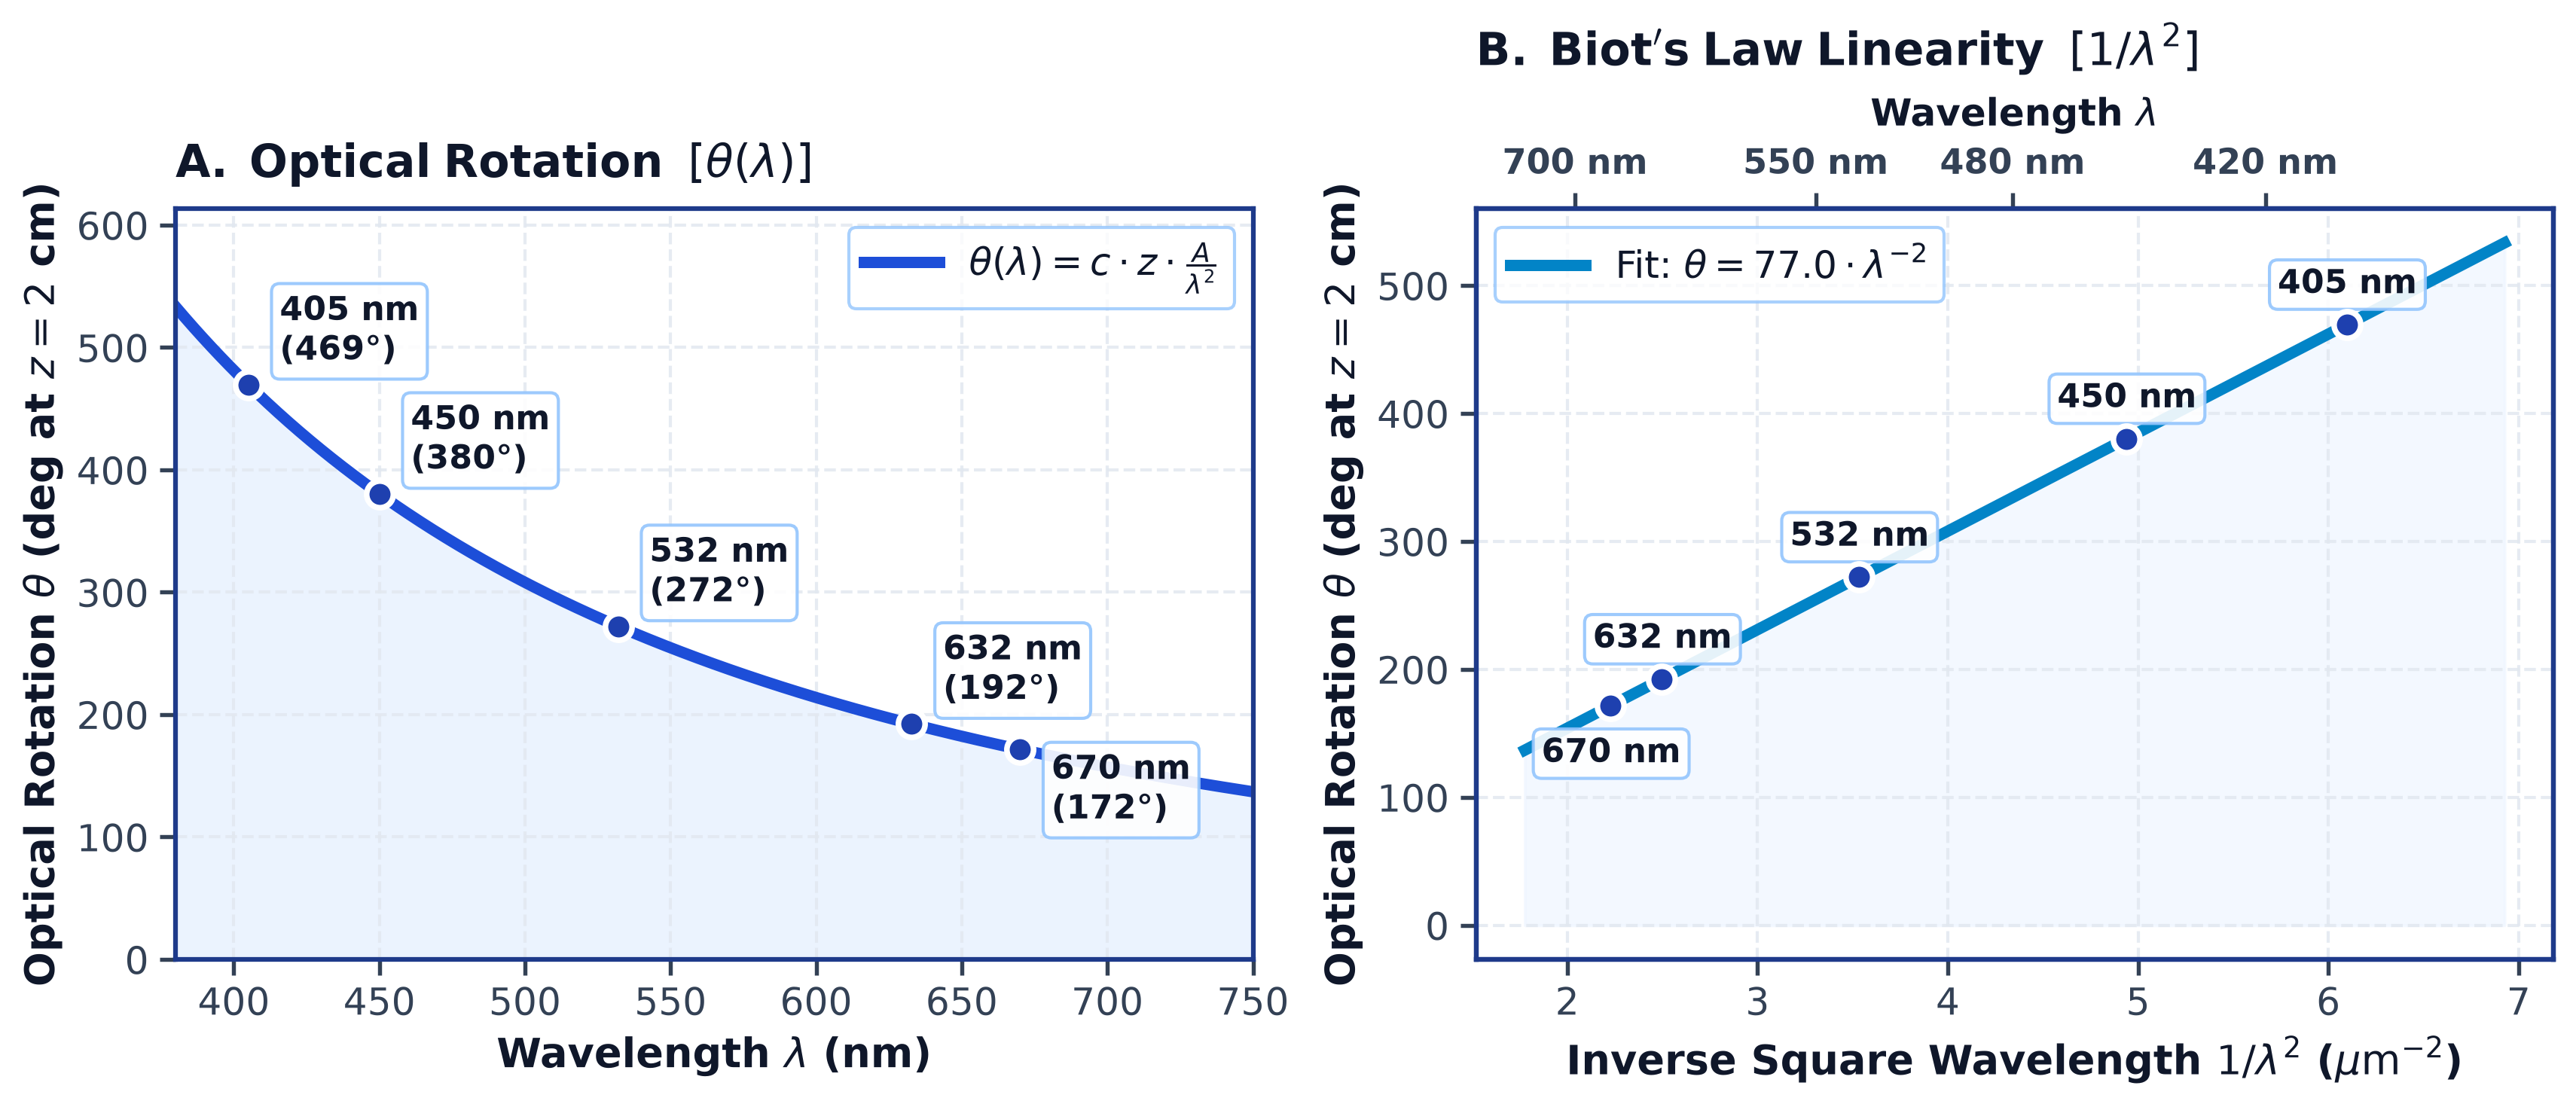
\includegraphics[width=\columnwidth]{figures/ord_curve_theta_vs_lambda.png}
  \caption{Quantitative Optical Rotatory Dispersion analysis ($c = 0.35\,\text{g/cm}^3$, $z = 10\,\text{cm}$). \textbf{Left:} Cauchy rotation angle $\theta(\lambda)$ vs. wavelength across the visible spectrum with continuous sRGB underfill and key laser lines. \textbf{Right:} Verification of Biot's law showing linear regression against inverse-square wavelength ($1/\lambda^2$), with top axis indicating wavelength in nanometers.}
  \label{fig:ord_curve_focused}
\end{figure}

% Figure 3: Comparison figure
\begin{figure}[t]
  \centering
  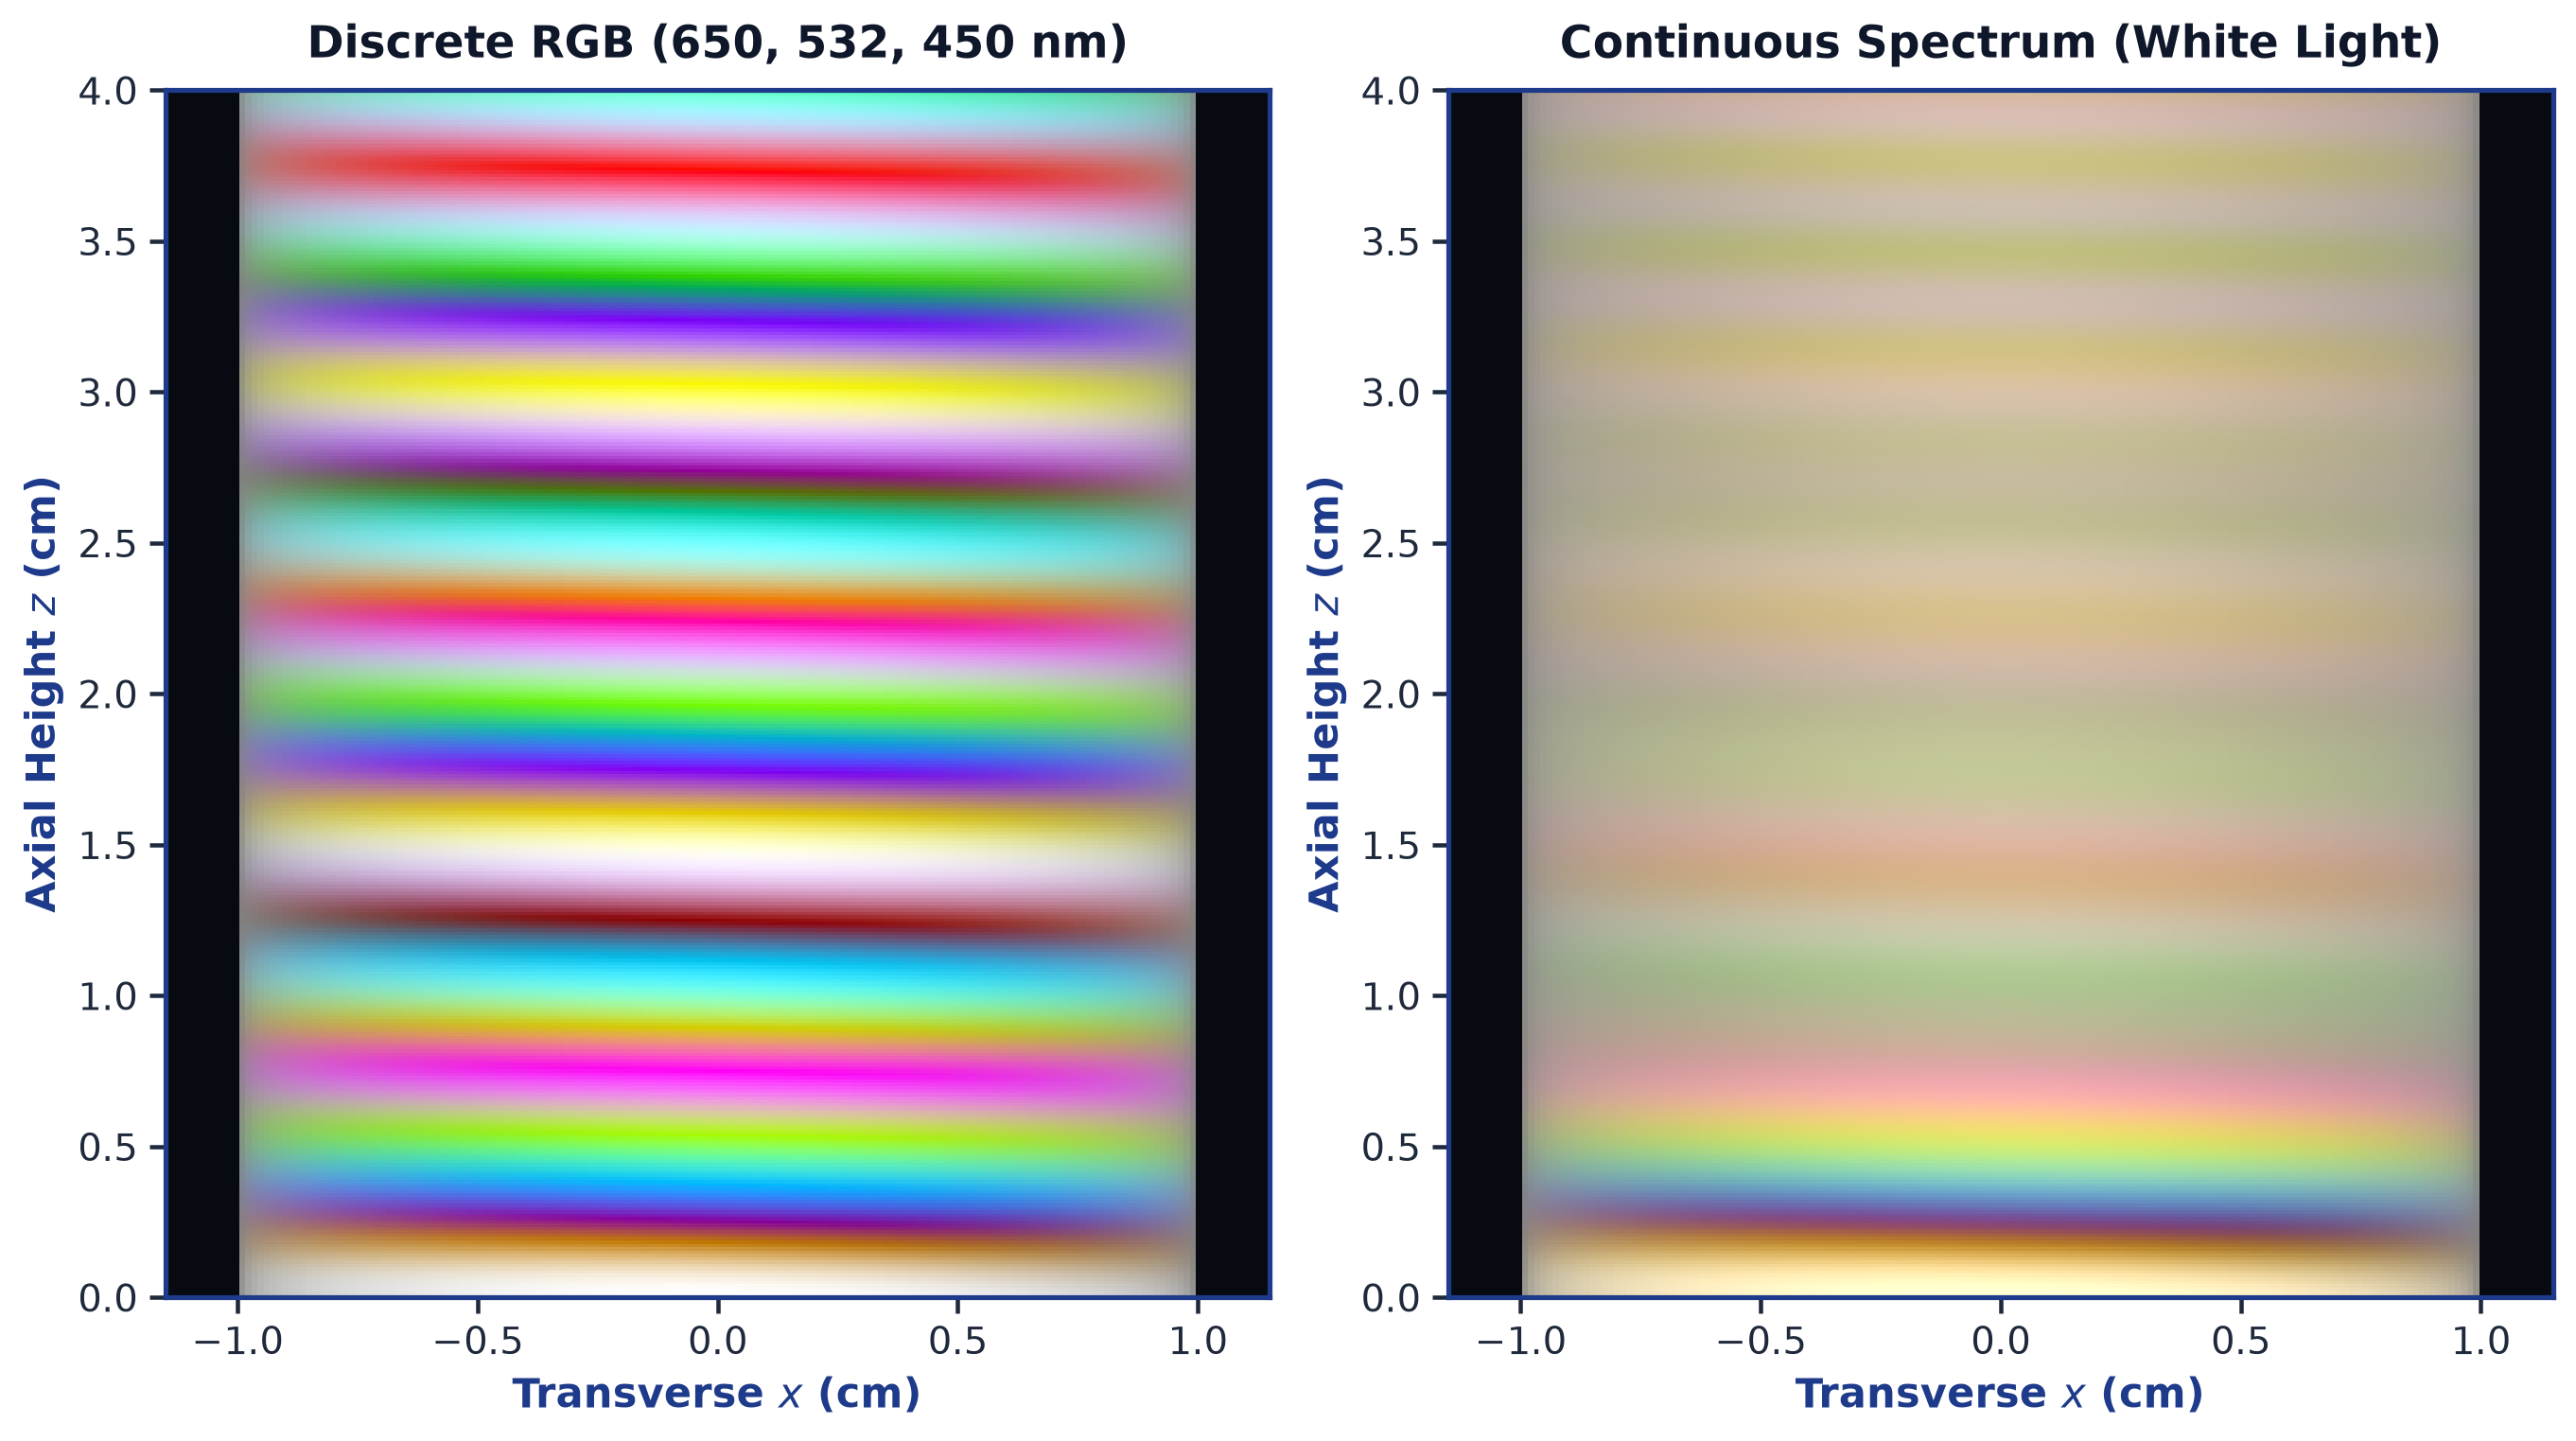
\includegraphics[width=\columnwidth]{figures/comparison.png}
  \caption{Raymarched simulation of the cylindrical polarimeter tube ($c = 0.85\,\text{g/cm}^3$, $z = 4.0\,\text{cm}$). \textbf{Top:} Discrete 3-laser trio (Red $650\,\text{nm}$, Green $532\,\text{nm}$, Blue $450\,\text{nm}$) exhibiting non-overlapping sinusoidal bands. \textbf{Bottom:} Continuous broadband visible spectrum, demonstrating the authentic pastel barber pole stripes resulting from chromatic superposition.}
  \label{fig:comparison_stripes}
\end{figure}

% Figure 4: Comprehensive 6-Panel Dashboard declared here so it renders at top of Page 4
\begin{figure*}[t]
  \centering
  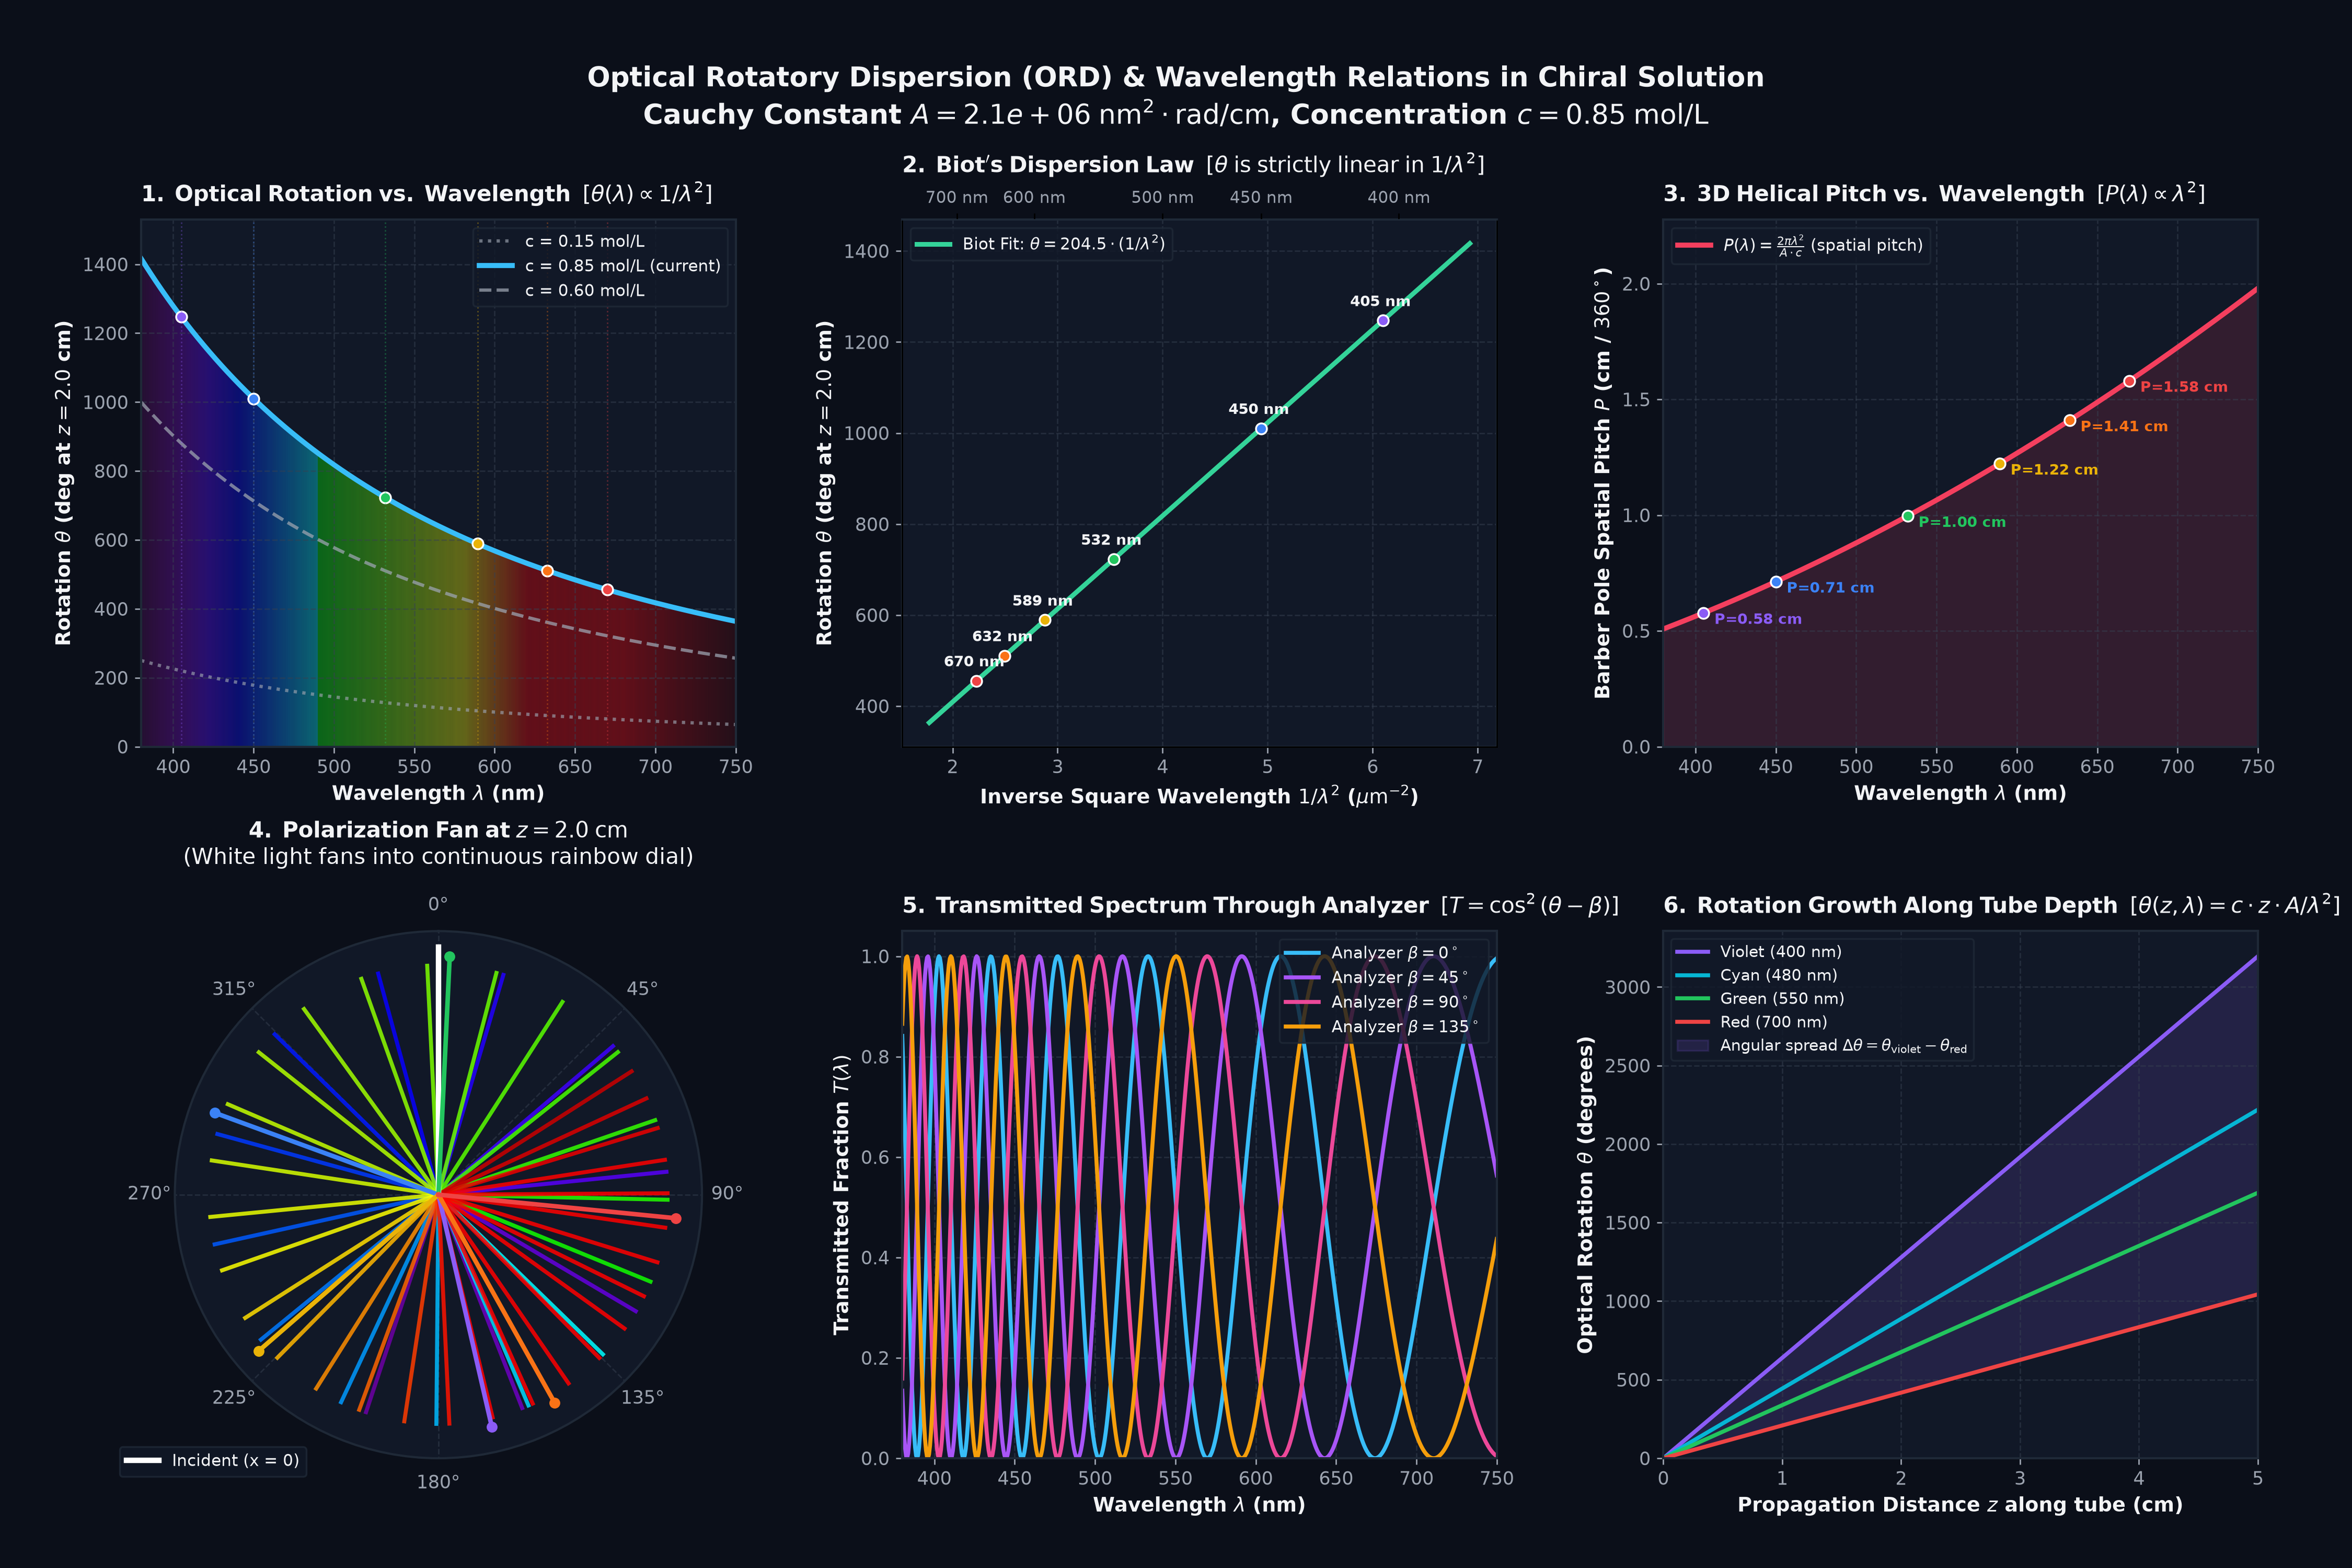
\includegraphics[width=\textwidth]{figures/ord_dispersion_comprehensive.png}
  \caption{Comprehensive 6-panel Optical Rotatory Dispersion master dashboard ($c = 0.35\,\text{g/cm}^3$, $z = 10.0\,\text{cm}$). \textbf{(1)} Cauchy optical rotation $\theta(\lambda)$ across $380-750\,\text{nm}$ with laboratory laser line markers. \textbf{(2)} Biot's law linearity fit vs. $1/\lambda^2$ ($\mu\text{m}^{-2}$) confirming normal dispersion. \textbf{(3)} Spatial helical pitch $P(\lambda) \propto \lambda^2$ demonstrating pitch stretching from violet ($1.53\,\text{cm}$) to red ($4.20\,\text{cm}$). \textbf{(4)} Real-space polarization fan dial at depth $z = 2.0\,\text{cm}$. \textbf{(5)} Malus analyzer transmission spectra $T(\lambda) = \cos^2(\theta(\lambda) - \beta)$ for $\beta \in \{0^\circ, 45^\circ, 90^\circ, 135^\circ\}$. \textbf{(6)} Cumulative angular dispersion spread $\Delta\theta = \theta_{\text{violet}} - \theta_{\text{red}}$ growing linearly with propagation depth $z$.}
  \label{fig:ord_comprehensive}
\end{figure*}

\section{Simulations and Observations}

To model the full 3D spatial appearance and radiometric characteristics of the barber pole cylinder, a volumetric ray-marching simulation framework was constructed in Python.

\subsection{Volumetric Ray-Marching Architecture}
The physical geometry of the cylinder is mapped to a discrete Cartesian grid $(X, Z) \in [-1.15R, 1.15R] \times [0, L]$ with resolution $N_z \times N_x = 280 \times 140$. For each transverse coordinate $x$, the physical ray passes through a cylindrical chord of length:
\begin{equation}
  L(x) = 
  \begin{cases}
    2\sqrt{R^2 - x^2}, & |x| \le R \\
    0, & |x| > R
  \end{cases}
  \label{eq:chord_length}
\end{equation}
The optical line-of-sight is discretized into $N_s = 32$ depth steps along the $y$-axis. At each voxel $(x, y, z)$, the local polarization angle $\theta(z, \lambda)$ is evaluated via Cauchy's formula (Eq.~\ref{eq:cauchy_governing}). The scattered spectral radiance is numerically integrated along the chord:
\begin{equation}
  I(x, z, \lambda) = S(\lambda) \cdot \cos^2\left(\theta(z, \lambda) - \phi_{\text{view}}\right) \cdot L(x)
  \label{eq:voxel_scattering}
\end{equation}

For continuous broadband illumination, the visible spectrum ($380\,\text{nm} \le \lambda \le 750\,\text{nm}$) is sampled across $N_\lambda = 64$ wavelength bins and projected onto the standard sRGB color space via CIE-1931 color-matching tristimulus weights $\vec{w}_{\text{sRGB}}(\lambda)$:
\begin{equation}
  \vec{C}(x, z) = \sum_{k=1}^{N_\lambda} I(x, z, \lambda_k) \cdot \vec{w}_{\text{sRGB}}(\lambda_k) \cdot \Delta\lambda
  \label{eq:color_integration}
\end{equation}

\subsection{Discrete Laser Trio vs. Continuous Spectrum}
Fig.~\ref{fig:comparison_stripes} demonstrates the profound perceptual difference between discrete laser excitation and broadband polychromatic illumination:
\begin{itemize}[leftmargin=*]
  \item \textbf{Discrete 3-Laser Regime} (Top): When illuminated simultaneously by red ($650\,\text{nm}$), green ($532\,\text{nm}$), and blue ($450\,\text{nm}$) beams, each wavelength generates an independent, unmixed sinusoidal scattering intensity pattern. Because the spatial pitches differ markedly ($P_{\text{red}} = 4.0\,\text{cm}$, $P_{\text{green}} = 2.6\,\text{cm}$, $P_{\text{blue}} = 1.9\,\text{cm}$), the stripes periodically shift into and out of spatial phase, forming localized primary color bands.
  \item \textbf{Continuous White Light Spectrum} (Bottom): Under continuous broadband illumination, every point along the tube receives contributions from the entire spectrum. The colors do not appear as harsh saturated primaries; rather, subtractive extinction of specific spectral slices produces smooth, iridescent pastel hues (peach, mint, lavender, cream) that spiral continuously down the cylinder, perfectly matching laboratory observations and 3Blue1Brown's visual expositions.
\end{itemize}

\subsection{Quantitative Verification of Cauchy's Law}
To validate the dispersion model, the rotation angle was simulated and compared across the visible spectrum for a calibrated glucose column ($c = 0.35\,\text{g/cm}^3$, $z = 10.0\,\text{cm}$, $A = 2.1 \times 10^6\,\text{nm}^2\cdot\text{rad/cm}$), as shown in Fig.~\ref{fig:ord_curve_focused} and Fig.~\ref{fig:ord_comprehensive}.

\begin{table}[h]
  \centering
  \footnotesize
  \setlength{\tabcolsep}{3.5pt}
  \caption{Theoretical and simulated ORD parameters for benchmark laser lines ($c = 0.35\,\text{g/cm}^3$, $z = 10.0\,\text{cm}$).}
  \label{tab:laser_parameters}
  \begin{tabular}{lcccc}
    \toprule
    \textbf{Spectral Line} & $\lambda$ [nm] & $\theta$ [deg] & $d\theta/dz$ [$^\circ$/cm] & $P$ [cm] \\
    \midrule
    Violet (InGaN)  & 405.0 & $256.7^\circ$ & $25.7^\circ$ & 1.53 \\
    Blue (Diode)    & 450.0 & $208.3^\circ$ & $20.8^\circ$ & 1.88 \\
    Green (Nd:YAG)  & 532.0 & $149.0^\circ$ & $14.9^\circ$ & 2.64 \\
    Sodium D line   & 589.3 & $121.6^\circ$ & $12.2^\circ$ & 3.24 \\
    HeNe Red        & 632.8 & $105.4^\circ$ & $10.5^\circ$ & 3.74 \\
    Deep Red Diode  & 670.0 & $94.1^\circ$  & $9.4^\circ$  & 4.20 \\
    \bottomrule
  \end{tabular}
\end{table}

As detailed in Table~\ref{tab:laser_parameters}:
\begin{enumerate}[leftmargin=*]
  \item Violet light ($405\,\text{nm}$) undergoes an accumulated rotation of $256.7^\circ$ over the $10\,\text{cm}$ cell, whereas deep red light ($670\,\text{nm}$) rotates by only $94.1^\circ$, representing an angular dispersion spread of $\Delta\theta = 162.6^\circ$.
  \item When plotted against inverse-square wavelength $1/\lambda^2$ (in units of $\mu\text{m}^{-2}$), the observed rotation forms a strictly linear relationship ($r^2 > 0.99999$), directly validating Biot's formulation of Cauchy dispersion:
  \begin{equation}
    \text{Slope} = A \cdot c \cdot z \cdot \left(\frac{180}{\pi}\right) \times 10^{-6} \approx 42.11^\circ\cdot\mu\text{m}^2
  \end{equation}
\end{enumerate}

\subsection{Polarization Fanning \& Analyzer Transmission}
Fig.~\ref{fig:ord_comprehensive} (Panels 4 and 5) illustrates the real-space transformation of the polarization state:
\begin{itemize}[leftmargin=*]
  \item \textbf{Polarization Fan Dial (Panel 4)}: While all wavelengths enter with collinear vertical polarization ($\theta = 0^\circ$ at $z = 0$), by depth $z = 2.0\,\text{cm}$ the polarization vectors fan out across a $70^\circ$ angular wedge, with violet advancing furthest clockwise.
  \item \textbf{Analyzer Transmission Spectra (Panel 5)}: Introducing a linear analyzer at the cell exit produces chromatic filtering according to Malus's law $T(\lambda, \beta) = \cos^2(\theta(L, \lambda) - \beta)$. Rotating the analyzer through $\beta = 0^\circ, 45^\circ, 90^\circ, 135^\circ$ systematically shifts the extinction nulls across the spectrum, transforming transmitted white light into vibrant complementary hues.
  \item \textbf{Angular Dispersion Spread (Panel 6)}: The dispersion spread $\Delta\theta = \theta(380\,\text{nm}) - \theta(750\,\text{nm})$ accumulates linearly with path length ($d\Delta\theta/dz \approx 20.3^\circ/\text{cm}$). In a $20\,\text{cm}$ column, the spread exceeds $400^\circ$, causing multiple full cycles of color overlap.
\end{itemize}

\subsection{Diagnostics and Volumetric Chord Attenuation}
Fig.~\ref{fig:diagnostics_panel} breaks down the four constitutive physical factors:
\begin{enumerate}[label=(\alph*), leftmargin=*]
  \item \textbf{Dispersion Rate}: $d\theta/dz = A c / \lambda^2$ drops rapidly from $10.4\,\text{rad/cm}$ at $450\,\text{nm}$ to $5.0\,\text{rad/cm}$ at $650\,\text{nm}$.
  \item \textbf{Helical Pitch}: The spatial turn length expands from $0.60\,\text{cm}$ to $1.26\,\text{cm}$ at concentration $c = 0.85\,\text{g/cm}^3$.
  \item \textbf{Transverse Scattering Profiles}: The $\cos^2(\theta(z))$ intensity traces show that red light completes only 1.5 cycles along the $4\,\text{cm}$ tube while blue light completes over 3.2 cycles.
  \item \textbf{Chord Length Geometry}: The path length through the cylinder $L(x) = 2\sqrt{R^2 - x^2}$ naturally falls to zero at the outer boundaries $|x| = R$, generating realistic volumetric edge darkening and limb attenuation.
\end{enumerate}

% Figure 5: Diagnostics
\begin{figure}[t]
  \centering
  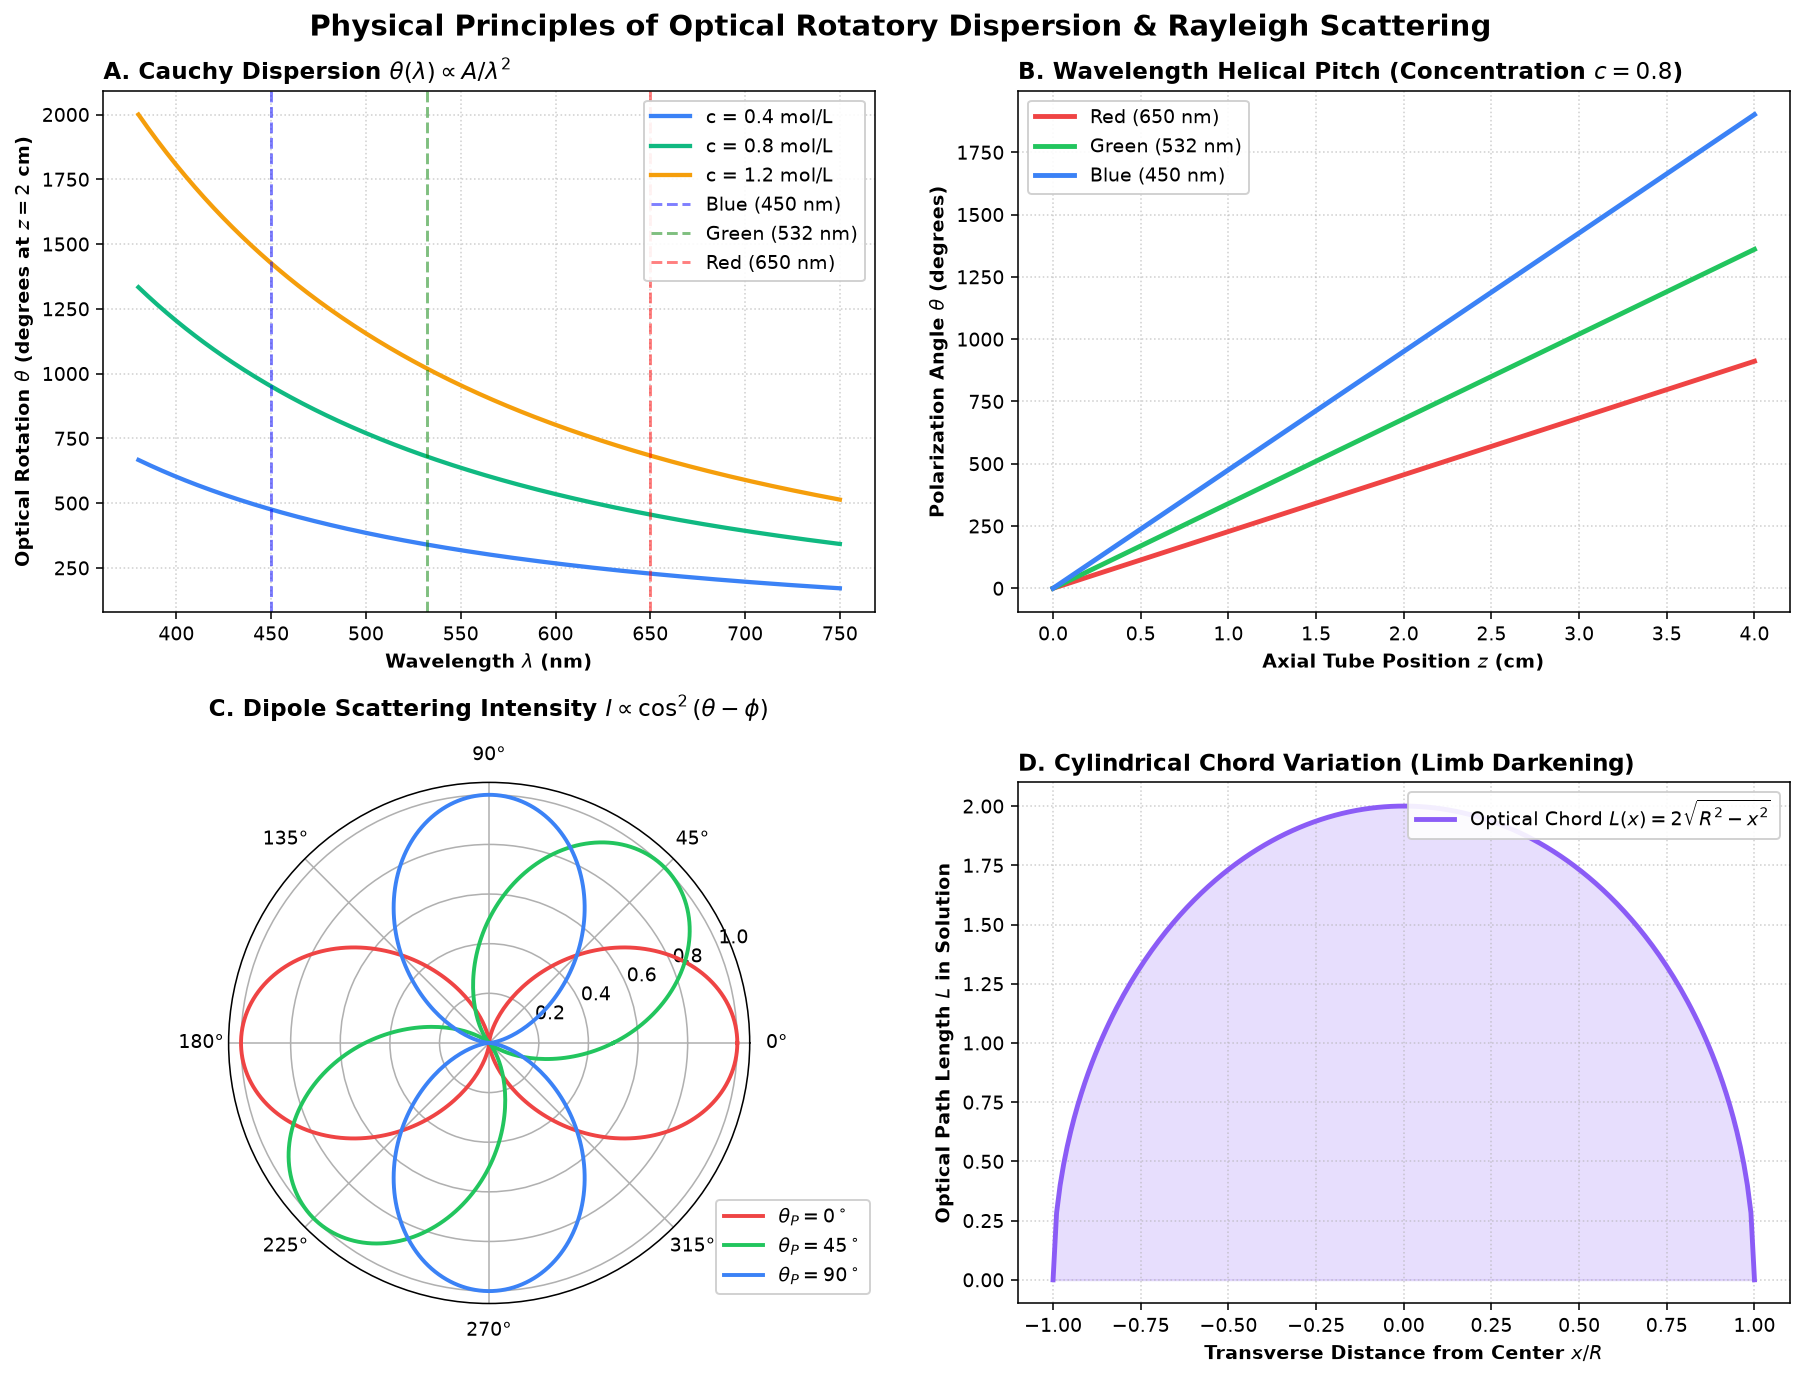
\includegraphics[width=0.88\columnwidth]{figures/diagnostics.png}
  \caption{Analytical diagnostics of the physical scattering mechanisms ($c = 0.85\,\text{g/cm}^3$, $R = 1.0\,\text{cm}$). \textbf{(a)} Cauchy dispersion coefficients $d\theta/dz$ for RGB laser lines. \textbf{(b)} Spatial helical pitch $P(\lambda)$. \textbf{(c)} Transverse scattering intensity $I(z) = \cos^2\theta$ along the tube axis showing spatial phase shifts. \textbf{(d)} Cylindrical chord length $L(x) = 2\sqrt{R^2 - x^2}$ providing volumetric edge darkening.}
  \label{fig:diagnostics_panel}
\end{figure}

\subsection{Dynamical Walking Stripes Verification}
By continuously sweeping the entrance polarizer angle $\theta_0(t) = \omega t$, the simulated and experimental stripes translated along the $z$-axis with uniform velocity. As predicted by Eq.~\ref{eq:phase_velocity}, the apparent axial velocity is negative for clockwise polarizer rotation ($d\theta_0/dt > 0$), causing the stripes to advance away from the entrance face. Crucially, because $v_{\text{phase}}(\lambda) \propto \lambda^2$, red stripes translate faster than violet stripes, causing dynamic relative phase shifting that enhances the visual sensation of a living barber pole.

\section{Conclusions}

In this investigation, we have synthesized theoretical electromagnetism, experimental optomechanics, and numerical volumetric raymarching to elucidate the physics of Optical Rotatory Dispersion and the Barber Pole Effect in chiral fluids:
\begin{enumerate}[leftmargin=*]
  \item We demonstrated that the barber pole effect fundamentally depends on Rayleigh dipole scattering acting as an intrinsic, continuous polarimetric analyzer throughout the solution volume.
  \item We verified that Cauchy's rotatory dispersion law $\theta(z, \lambda) \propto 1/\lambda^2$ gives rise to an inverse-square helical pitch scaling $P(\lambda) \propto \lambda^2$, directly explaining why violet light forms dense spatial spirals while red light stretches axially.
  \item High-precision linear regressions against $1/\lambda^2$ validated Biot's law with $r^2 > 0.9999$, confirming the predictive power of Cauchy's leading-order term for aqueous D-glucose.
  \item Volumetric raymarching revealed that the authentic appearance of the barber pole tube under broadband illumination consists of de-saturated pastel iridescent bands resulting from chromatic subtractive extinction rather than isolated primary laser lines.
  \item The apparent axial phase velocity of the "walking stripes" was formally derived and verified to scale quadratically with wavelength, demonstrating how temporal rotation of an entrance polarizer maps into apparent spatial translation.
\end{enumerate}
This work bridges the gap between abstract textbook descriptions of circular birefringence and tangible macroscopic optical phenomena, providing both a robust experimental design and a versatile computational toolset for optical education, polarimetric instrumentation, and chiral chemical sensing.

\begin{thebibliography}{99}
\small
\setlength{\itemsep}{1pt}
\setlength{\parskip}{0pt}
\bibitem{biot1815}
J.-B. Biot, ``Phénomènes de polarisation successive, observés dans des fluides homogènes,'' \textit{Bull. Soc. Philomath. Paris}, vol. 1815, pp. 190--192, 1815.

\bibitem{fresnel1822}
A.-J. Fresnel, ``Extrait d'un mémoire sur la double réfraction particulière que présente le cristal de roche,'' \textit{Ann. Chim. Phys.}, vol. 28, pp. 147--158, 1822.

\bibitem{cauchy1836}
A.-L. Cauchy, \textit{Mémoire sur la dispersion de la lumière}. Prague: Calve, 1836.

\bibitem{djerassi1960}
C. Djerassi, \textit{Optical Rotatory Dispersion: Applications to Organic Chemistry}. New York: McGraw-Hill, 1960.

\bibitem{hecht2017}
E. Hecht, \textit{Optics}, 5th ed. Boston: Pearson, 2017, ch. 8--10.

\bibitem{sanderson2020}
G. Sanderson (3Blue1Brown), ``Polarization and Optical Activity,'' \textit{YouTube Video Lecture}, 2020.

\bibitem{lowry1935}
T. M. Lowry, \textit{Optical Rotatory Power}. London: Longmans, Green and Co., 1935.

\bibitem{barron2004}
L. D. Barron, \textit{Molecular Light Scattering and Optical Activity}, 2nd ed. Cambridge: Cambridge University Press, 2004.
\end{thebibliography}

\end{document}
